% Created 2021-05-07 Fri 22:57
% Intended LaTeX compiler: pdflatex
\documentclass[11pt]{article}
\usepackage[utf8]{inputenc}
\usepackage[T1]{fontenc}
\usepackage{graphicx}
\usepackage{grffile}
\usepackage{longtable}
\usepackage{wrapfig}
\usepackage{rotating}
\usepackage[normalem]{ulem}
\usepackage{amsmath}
\usepackage{textcomp}
\usepackage{amssymb}
\usepackage{capt-of}
\usepackage{hyperref}
\usepackage{minted}
\usepackage{tabularx}
\author{Philipp Beer}
\date{2021-05-10}
\title{592 Project Report}
\hypersetup{
 pdfauthor={Philipp Beer},
 pdftitle={592 Project Report},
 pdfkeywords={unic, 501dl, stassopoulou},
 pdfsubject={project report presentation of time series clustering},
 pdfcreator={Emacs 27.2 (Org mode 9.4)}, 
 pdflang={English}}
\begin{document}

\maketitle


\section*{Clustering M4 Daily Data for Forecasting}
\label{sec:orgd3b6979}
\url{https://552dlimages.s3-eu-west-1.amazonaws.com/unic\_logo.png}

Philipp Beer\\
Gradudate Program Data Science, UNIC

COMP-501DL Research\\
Prof. Spyros Makridakis \& Prof. Ioannis Katakis\\
\subsection*{Introduction}
\label{sec:org088bb96}
\subsubsection*{M4 Competition Forecasting}
\label{sec:orgdcd1239}
\begin{itemize}
\item say something here
\end{itemize}

\subsubsection*{Machine Learning in time series forecasting}
\label{sec:orgbf9174a}
\begin{itemize}
\item regularly outperformed by M4 competition benchmark
\item high computational costs
\item few data points for time series
\end{itemize}
\subsubsection*{Grouping similar time series}
\label{sec:org90849ae}
\begin{itemize}
\item combine series - more data to learn from
\item ts with similar properties
\item less complex learning task
\end{itemize}
\subsubsection*{Can it improve forecast performance}
\label{sec:org65bbf95}
\subsection*{Time Series  Properties}
\label{sec:orgcd83e92}
\subsubsection*{Feature Representation}
\label{sec:org3d565d8}
\begin{itemize}
\item shape-, feature-, model-based
\item extraction via Python software package tsfresh
\end{itemize}
\subsection*{Clustering}
\label{sec:org8dee5f5}
\begin{itemize}
\item unsupervised learning technique
\item learn from data without or minimal input
\end{itemize}
\subsubsection*{Philosophical view}
\label{sec:orgbc23086}
\begin{itemize}
\item segmentation
\item finding groups
\item means to find distinction
\end{itemize}
\subsubsection*{K-Means}
\label{sec:orge20e0b0}
\begin{itemize}
\item grouping unlabeled data into predetermined number of groups
\item random starting point of points
\item iterative adjustment
\end{itemize}
\subsection*{Deciding k}
\label{sec:orgafdd5ac}
\subsubsection*{Inertia}
\label{sec:org8426905}
goal: minimize within cluster sum-of-squares
  $$ \sum_{i=0}^n \min_{\mu_j \in C}(\lvert \lvert x_i - \mu_j \rvert \rvert^2) $$
\begin{center}
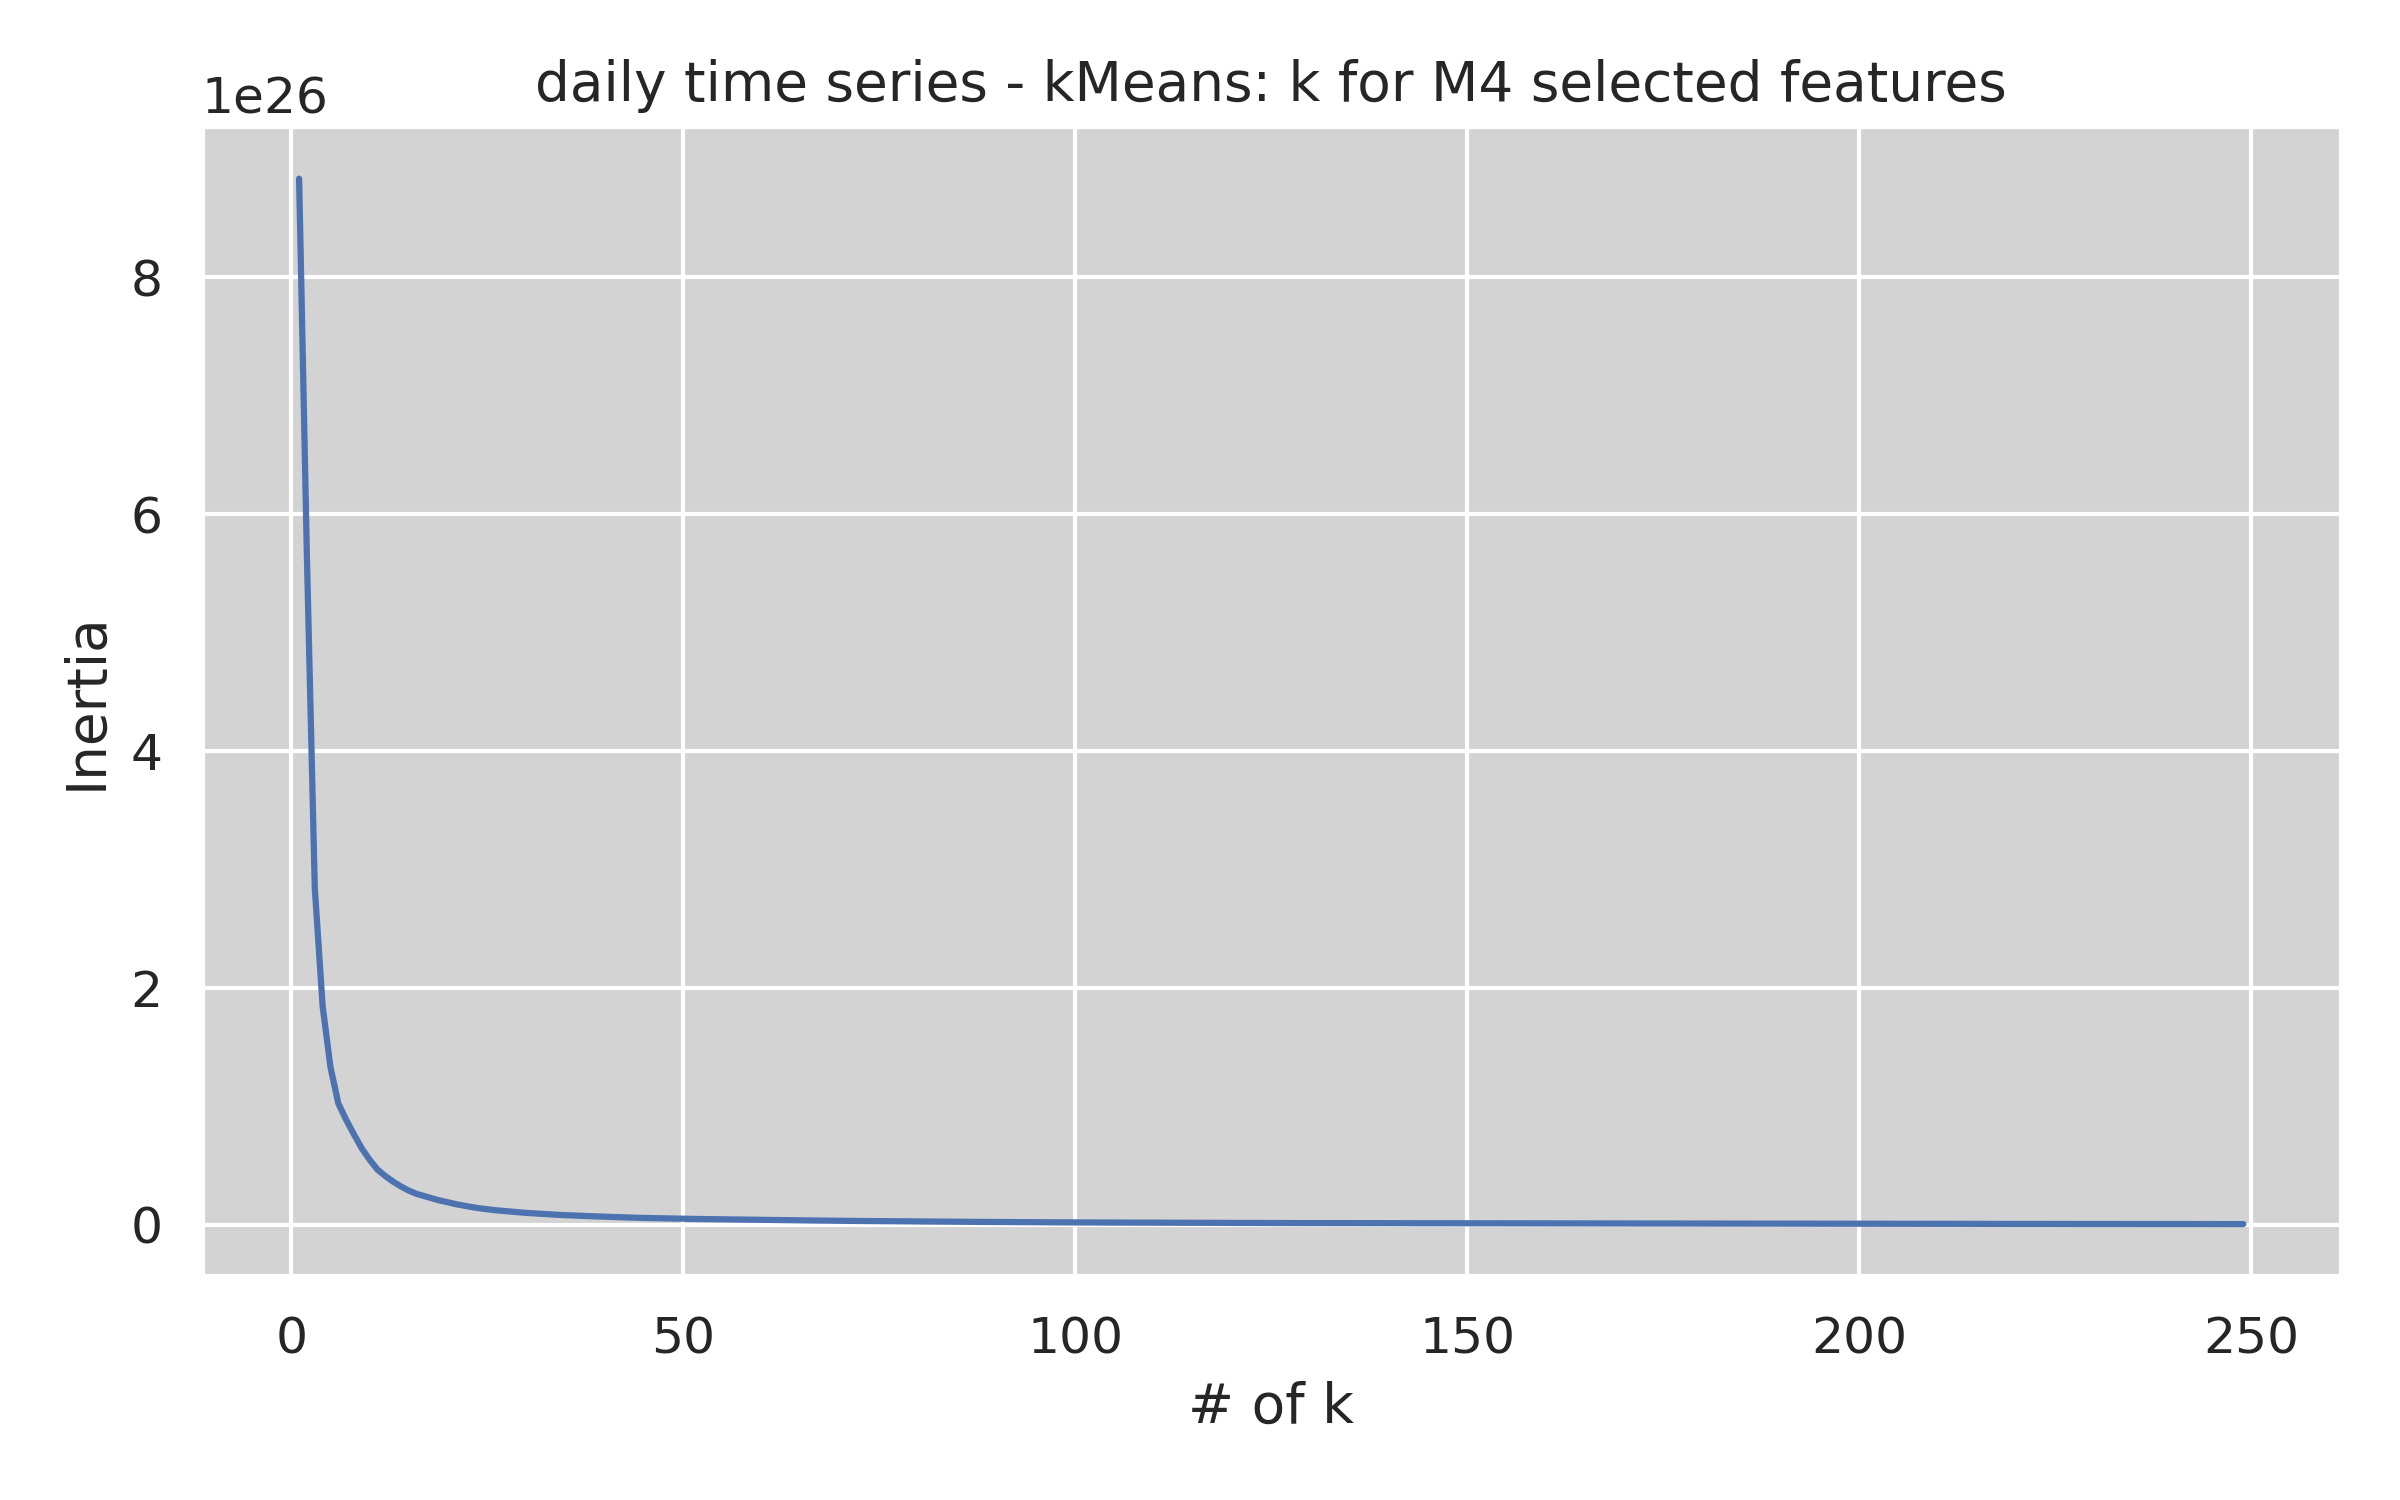
\includegraphics[width=500px]{../img/daily_kmeans_series_inertia.png}
\end{center}
\subsubsection*{Silhouette score}
\label{sec:orgb597cb8}
$$ s(i) = \frac{b(i) - a(i)}{{\max\{a(i),b(i)\}}} $$
  \begin{center}
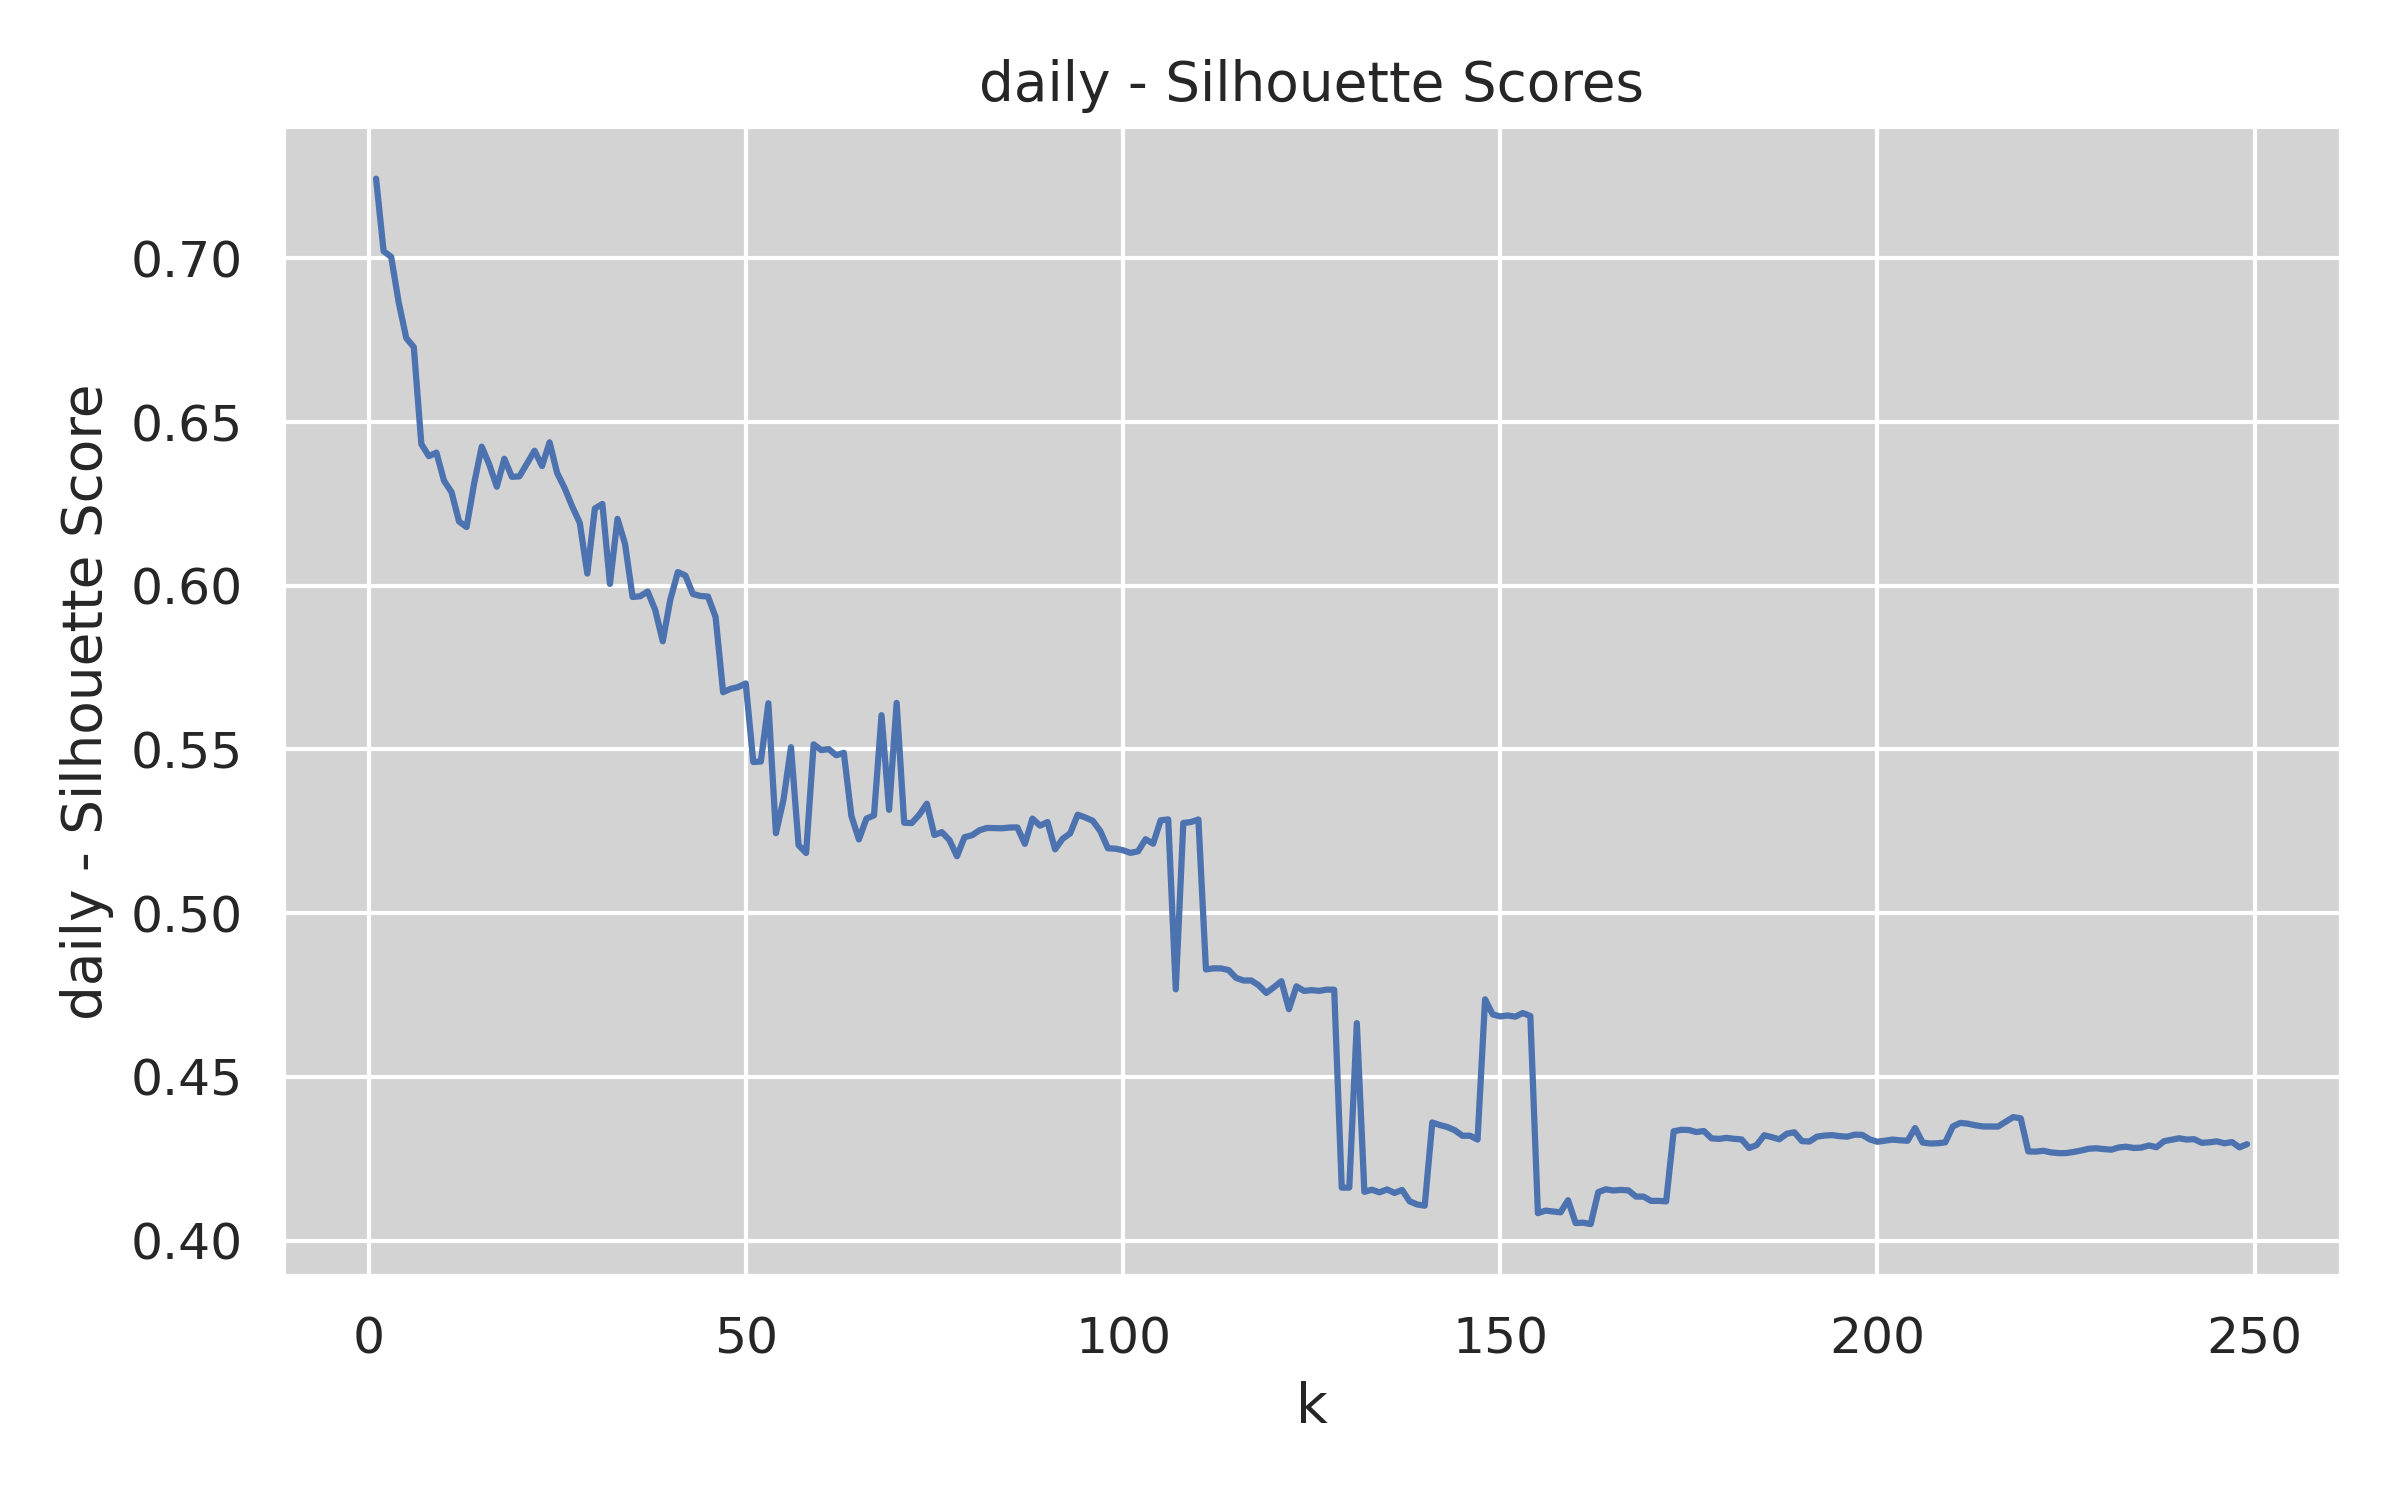
\includegraphics[width=.9\linewidth]{../img/daily_kmeans_sil_score_series.png}
\end{center}
\subsubsection*{Silhouette Diagrams}
\label{sec:org95e89f6}
\begin{center}
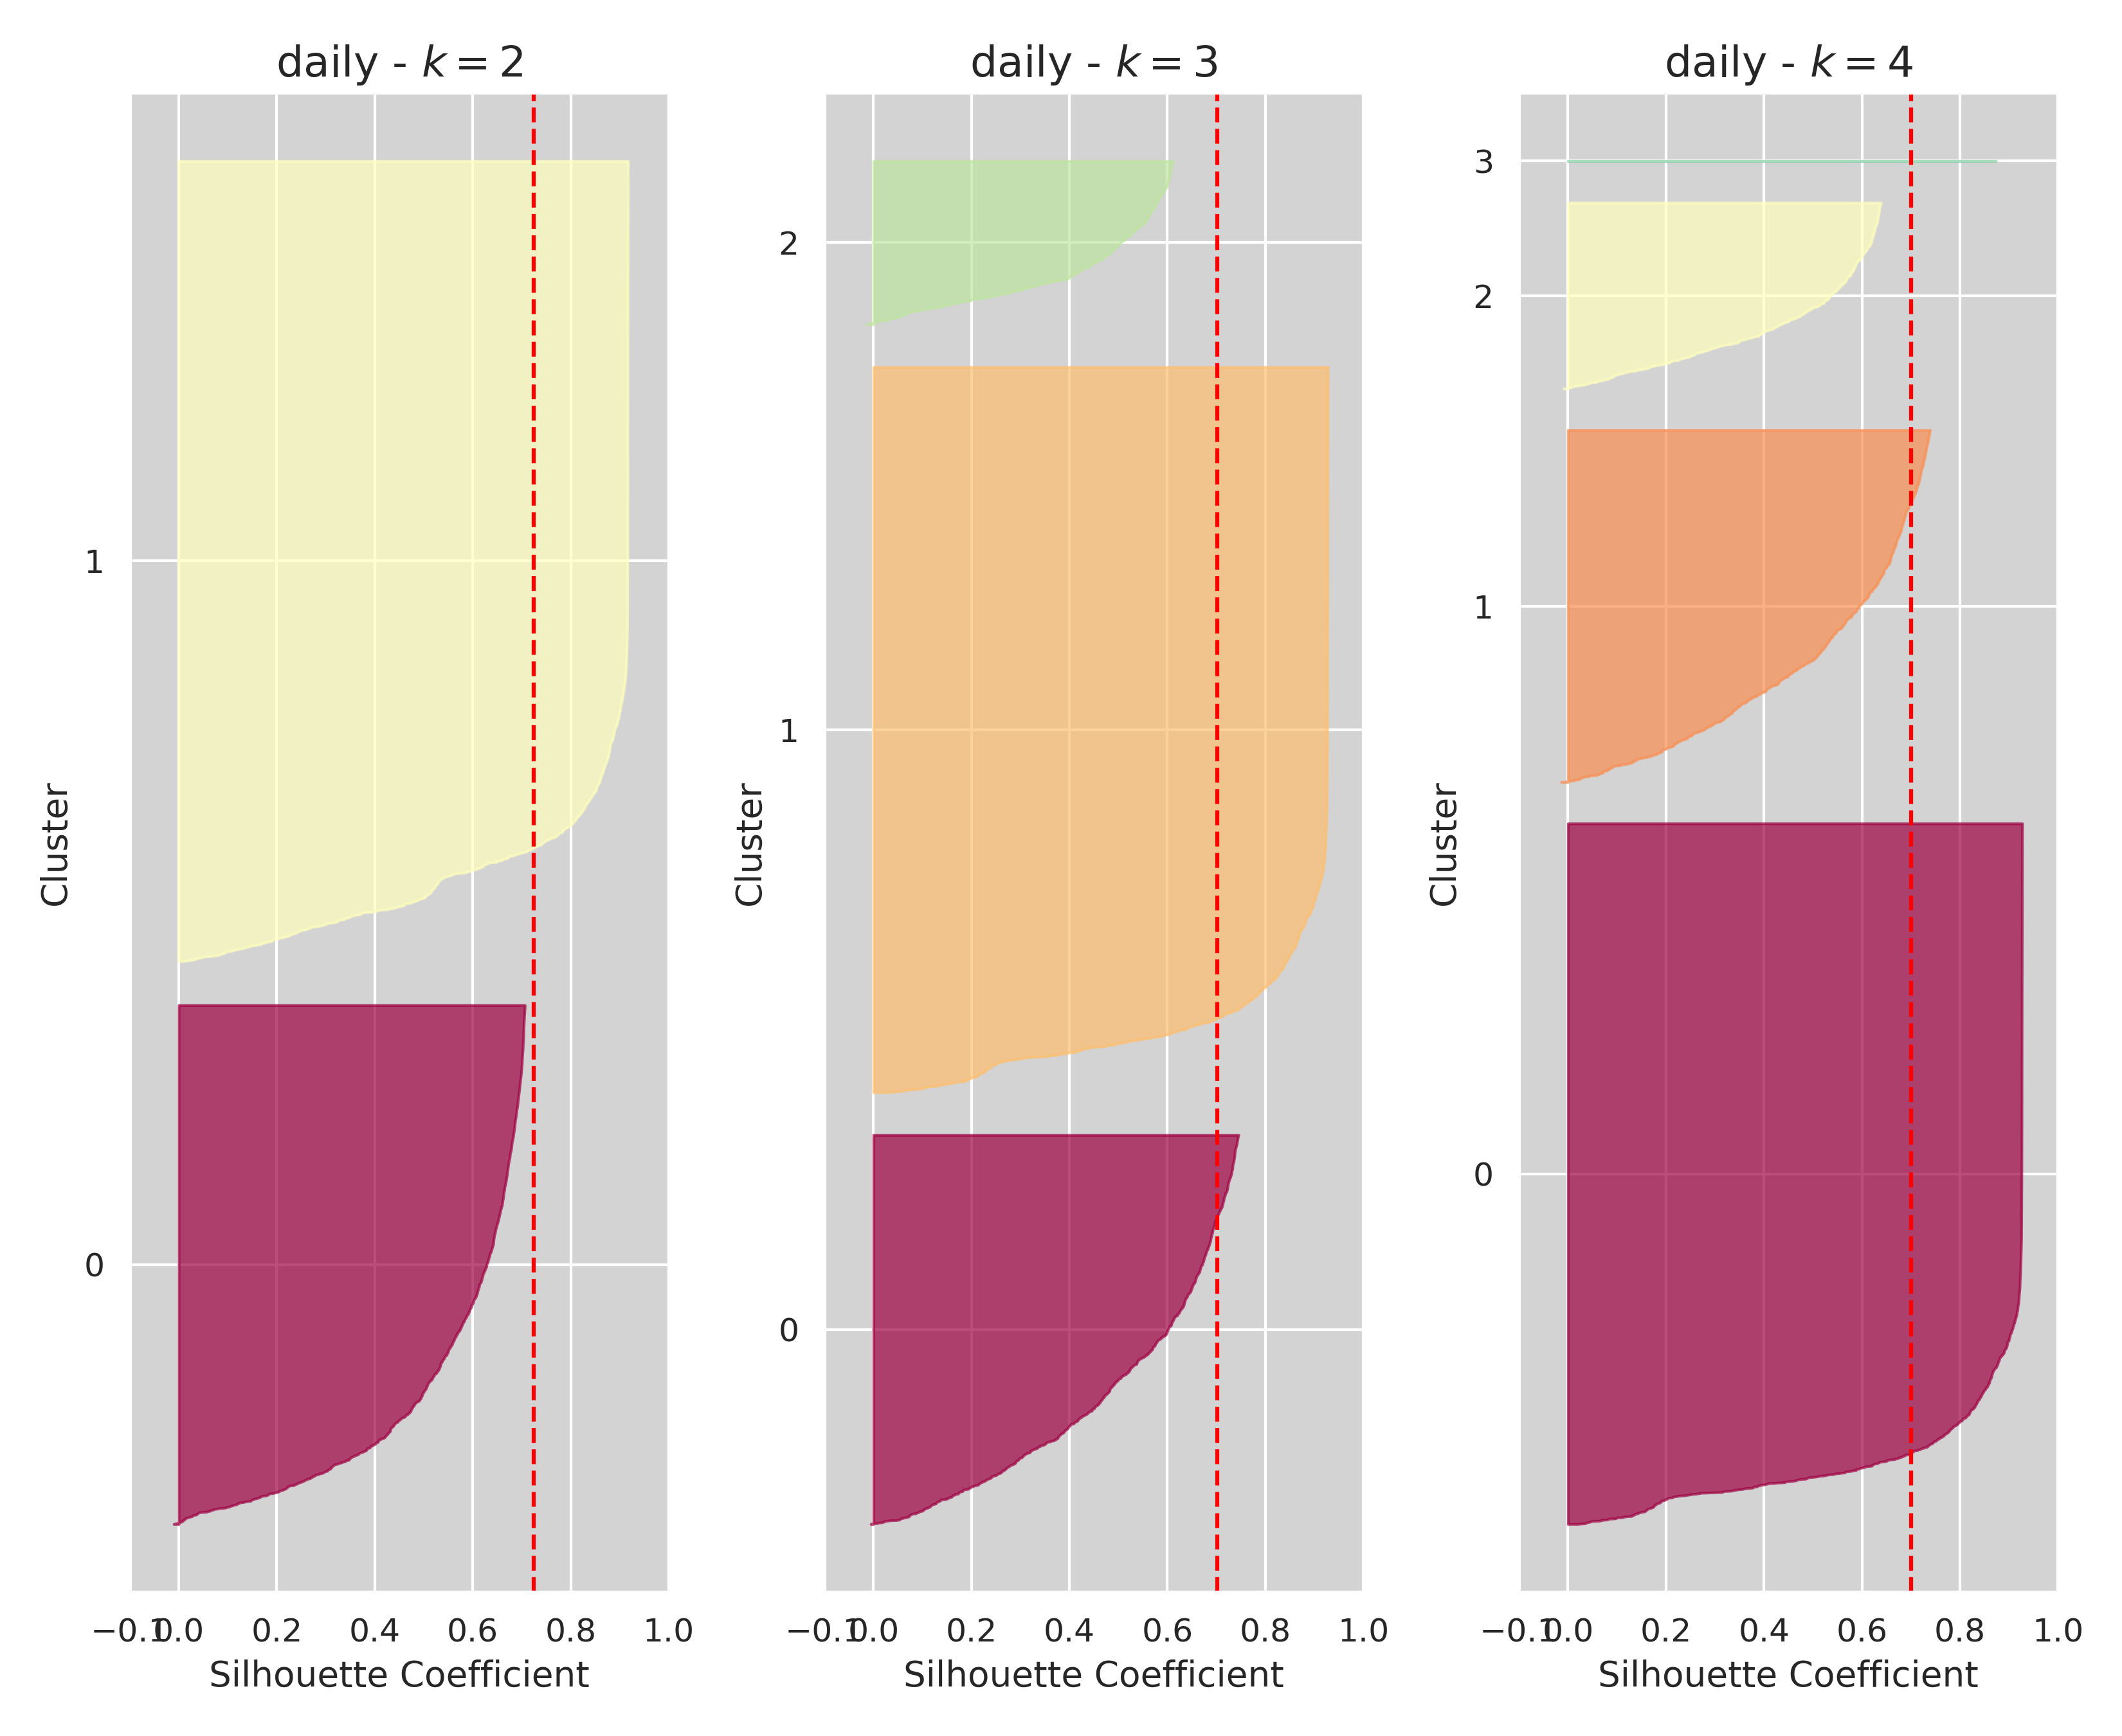
\includegraphics[width=.9\linewidth]{../img/daily_kmeans_sil_dia_series.png}
\end{center}
\subsection*{Forecasting}
\label{sec:orgea3d9ed}
\subsubsection*{Neural Network}
\label{sec:org4250d06}
\begin{itemize}
\item 3 hidden layers
\item features - lags 1 - 7
\item loss: MSE
$$ MSE = \frac{1}{n} \sum_{i=1}^n (Y_i - \hat{Y}_i)^2 $$
\end{itemize}
\subsubsection*{Approach}
\label{sec:org0b93389}
\begin{itemize}
\item full dataset
\item clustered datasets
\item equivalent random datasets
\end{itemize}
\subsubsection*{Cross-Validation}
\label{sec:orgcda258a}
\begin{itemize}
\item increase certainty about the error that is encountered in the training
\item limit effects of particularities in the data on error metrics
\end{itemize}
\subsection*{Benchmarking}
\label{sec:orga923736}
\subsubsection*{M4 Accuracy Metrics}
\label{sec:org52862e2}
$$ SMAPE = \frac{100}{n} \sum_{t=1}^{n} \frac{F_t - Y_t}{(\lvert F_t \rvert + \lvert Y_t \rvert)/2} $$
$$ MASE = mean \left( \frac{\lvert e_j \rvert}{\frac{1}{T-1} \sum_{t=2}^{T} \lvert Y_t - Y_{t-1} \rvert} \right) $$
\subsection*{Challenges}
\label{sec:orgd121099}
\subsubsection*{Data Preprocessing}
\label{sec:orgcab51b3}
\begin{itemize}
\item data format - wide vs. long format
\item Min-Max feature scaling with cross validation with neural networks
\item information leakage
\end{itemize}
\subsubsection*{Feature extraction and selection}
\label{sec:orgec68efa}
\begin{itemize}
\item tsfresh - 800 metrics
\item comprehensive vs. efficient
\end{itemize}
\subsubsection*{Computational Costs}
\label{sec:orgbd6a769}
\begin{itemize}
\item 6 vCPU / 32GB RAM
\item feature extraction and selection (reason for daily only)
\item neural network with cv
\end{itemize}

\subsection*{Results}
\label{sec:orgefcf33b}
\subsubsection*{Cross validation}
\label{sec:org9ecaa74}
\begin{center}
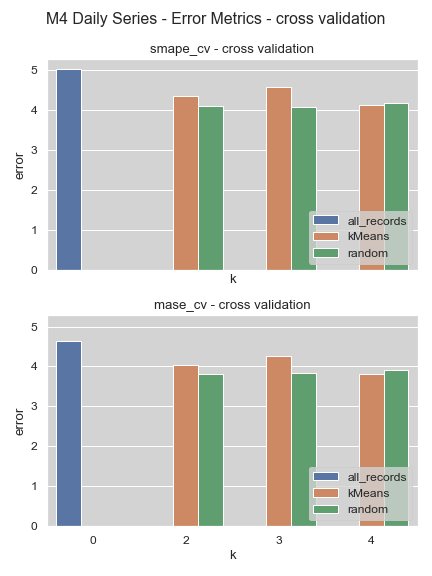
\includegraphics[width=.9\linewidth]{../img/daily_cv_results.png}
\end{center}
\subsubsection*{M4 results}
\label{sec:orgce1f6c8}
\begin{center}
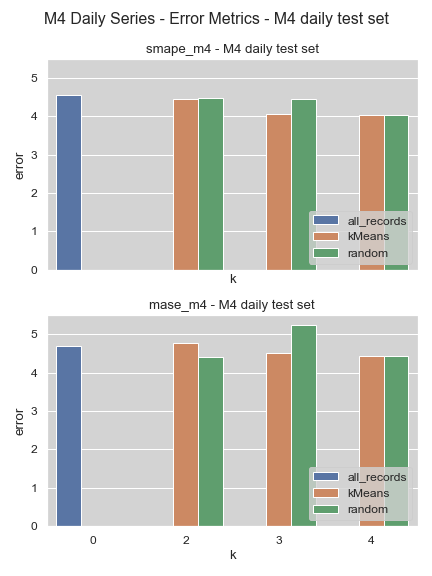
\includegraphics[width=.9\linewidth]{../img/daily_m4_results.png}
\end{center}
\subsection*{Conclusion}
\label{sec:org84c404d}
\begin{itemize}
\item clustering results not better than random
\end{itemize}
\subsubsection*{features vs lags for NN}
\label{sec:org965bd88}
\begin{itemize}
\item possibly better results
\item increase of neural network size
\item how meaningful are efficient features
\end{itemize}
\subsubsection*{Approach to cross validation}
\label{sec:orgdd3d84a}
\begin{itemize}
\item less folds
\item MinMax scaler
\end{itemize}
\subsubsection*{Uncertainty in the clustering}
\label{sec:orgd78a8d8}
\begin{itemize}
\item reduced uncertainty in the data clustered data
\item indication in MASE (higher in test results compared to cv)
\end{itemize}
\subsubsection*{Complexity of problem definition}
\label{sec:orgc5ae0e2}
\begin{itemize}
\item many moving parts
\item \href{https://github.com/philippbeer/m4\_clustering}{M4 Clustering on Github}
\end{itemize}
\subsection*{Outlook}
\label{sec:org347f478}
\subsubsection*{Algorithm}
\label{sec:org7e7f701}
\begin{itemize}
\item hierarchical and density and grid-based methods
\end{itemize}
\subsubsection*{Feature Choice}
\label{sec:orgd961f30}
\begin{itemize}
\item ranking of features
\end{itemize}
\end{document}